\tikzset{%
  neuron missing/.style={
    draw=none, 
    scale=4,
    text height=0.333cm,
    execute at begin node=\color{black}$\vdots$
  },
}
\def\X{1.5}
\hspace*{1.5cm}
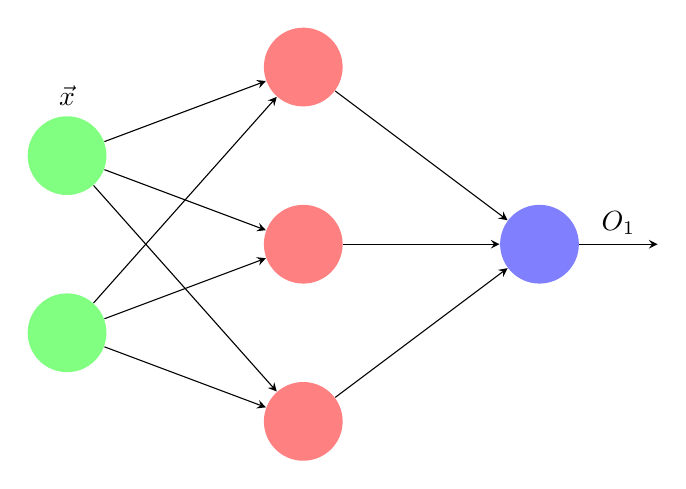
\begin{tikzpicture}[x=1.5cm, y=1.5cm, >=stealth]
  % draw input features  
  \foreach \m/\l [count=\y] in {1,2}
  {
    \node [circle,fill=green!50,minimum size=1cm] (input-\m) at (0, 1.25 - \X*\y) {};
  }
  
  % draw hidden layers
  \foreach \m [count=\y] in {1, 2, 3}
  \node [circle,fill=red!50,minimum size=1cm ] (hidden-\m) at (2, 2.0 - \X*\y) {};  
  
  % draw output neurons
  \foreach \m [count=\y] in {1}
  \node [circle,fill=blue!50,minimum size=1cm ] (output-\m) at (4, -1) {};

  \foreach \l [count=\i] in {1}
  \node [above] at (input-\i.north) {$\vec{x}$};
  

  \draw [->] (output-1) -- ++(1,0)
  node [above, midway] {$O_{1}$};

  \foreach \i in {1, 2}
  \foreach \j in {1,...,3}
  \draw [->] (input-\i) -- (hidden-\j);

  \foreach \i in {1,...,3}
  \draw [->] (hidden-\i) -- (output-1);

  % \foreach \l [count=\x from 0] in {Input, Hidden, Ouput}
  % \node [align=center, above] at (\x*2,2) {\l \\ layer};

\end{tikzpicture}
